\documentclass{article}
\usepackage{tikz}
\usetikzlibrary{arrows.meta,positioning,calc,shapes.geometric}
\pagestyle{empty}
\begin{document}
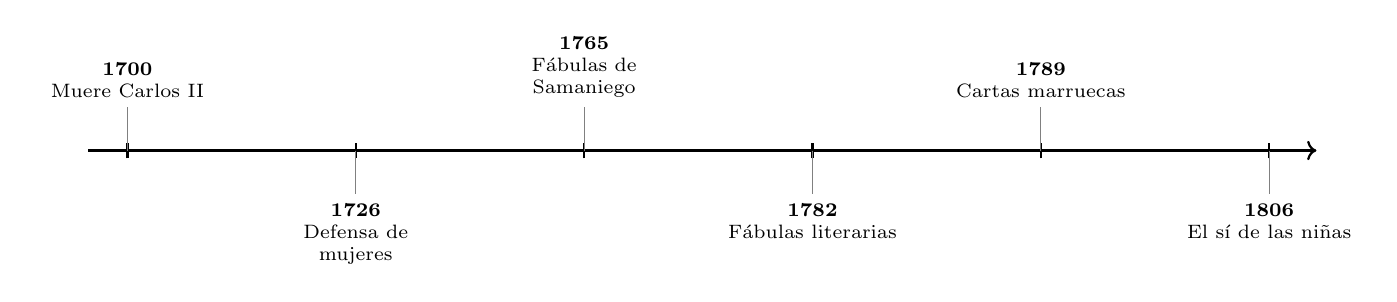
\begin{tikzpicture}
\tikzset{every node/.append style={align=center}}
\draw[->, thick] (-0.5,0) -- (15.10,0);
\draw[thick] (0.00,-0.1) -- (0.00,0.1);
\draw[gray] (0.00,0) -- (0.00,0.55);
\node[anchor=south, align=center, text width=2.30cm, font=\scriptsize] at (0.00,0.55) {\textbf{1700}\\ Muere Carlos II};
\draw[thick] (2.90,-0.1) -- (2.90,0.1);
\draw[gray] (2.90,0) -- (2.90,-0.55);
\node[anchor=north, align=center, text width=2.30cm, font=\scriptsize] at (2.90,-0.55) {\textbf{1726}\\ Defensa de mujeres};
\draw[thick] (5.80,-0.1) -- (5.80,0.1);
\draw[gray] (5.80,0) -- (5.80,0.55);
\node[anchor=south, align=center, text width=2.30cm, font=\scriptsize] at (5.80,0.55) {\textbf{1765}\\ Fábulas de Samaniego};
\draw[thick] (8.70,-0.1) -- (8.70,0.1);
\draw[gray] (8.70,0) -- (8.70,-0.55);
\node[anchor=north, align=center, text width=2.30cm, font=\scriptsize] at (8.70,-0.55) {\textbf{1782}\\ Fábulas literarias};
\draw[thick] (11.60,-0.1) -- (11.60,0.1);
\draw[gray] (11.60,0) -- (11.60,0.55);
\node[anchor=south, align=center, text width=2.30cm, font=\scriptsize] at (11.60,0.55) {\textbf{1789}\\ Cartas marruecas};
\draw[thick] (14.50,-0.1) -- (14.50,0.1);
\draw[gray] (14.50,0) -- (14.50,-0.55);
\node[anchor=north, align=center, text width=2.30cm, font=\scriptsize] at (14.50,-0.55) {\textbf{1806}\\ El sí de las niñas};
\end{tikzpicture}
\end{document}
